\section{2º/2017}
\begin{exercicio}
  {2º/2017}{Threads}
  {Por quê a implementação de \textit{threads} em nível de usuário possui um custo extremamente baixo de troca de contexto?}

  Comparando o custo da troca de contexto à nível de kernel com a implementação à nível \textit{threads}, o custo é extremamente baixo pois as trocas de contexto entre \textit{threads} não possuem o custo da troca de modo usuário para protegido, uma vez que esta troca é feita em nível de aplicação, existindo apenas no nível de usuário. À nível de \textit{threads} se resume a utilizar conjunto de instruções de \textit{load}, \textit{store} e \textit{jump} para simular uma troca de contexto, enquanto à nível kernel alterna entre modo usuário para protegido e modo usuário utilizando-se instruções de \textit{long jump}.
\end{exercicio}

\begin{exercicio}
  {2º/2017}{Condições de Corrida}
  {Defina condição de corrida. Considere o código multi-processo abaixo. Existe condição de corrida nesse código? Se sim, corrija o código de maneira a eliminá-la.
  \begin{figure}[H]
    \centering
    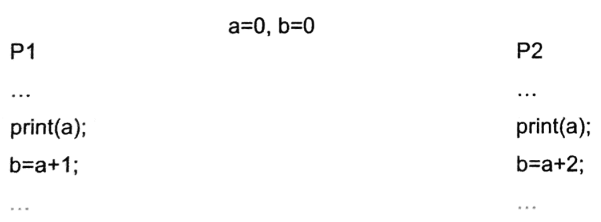
\includegraphics[width=0.5\textwidth]{ex-race-cond}
  \end{figure}}

  \textbf{Condição de Corrida:} quando dois ou mais processos acessam concorrentemente um recurso e o resultado final sobre este recurso depende da ordem na qual os processos foram executados.

  Sim, existe condição de corrida na variável $b$. Utilizamos \textit{locks} para a nossa solução:

  \begin{table}[H]
    \centering
    \begin{tabular}{l|l}
      \textbf{P1:}            & \textbf{P2:} \\
      \texttt{print(a)}       & \texttt{print(a)} \\
      \texttt{acquire(lock)}  & \texttt{acquire(lock)} \\
      \texttt{b = a + 1}      & \texttt{b = a + 2} \\
      \texttt{release(lock)}  & \texttt{release(lock)}\\
    \end{tabular}
  \end{table}
\end{exercicio}

\begin{exercicio}
  {2º/2017}{Deadlocks}
  {Por quê \textit{deadlocks} são ditos \textit{stable properties}?}

  Pois consistem em estados que não podem ser mudados sem utilização de força externa.
\end{exercicio}

\begin{exercicio}
  {2º/2017}{Arquivos}
  {Qual a função da operação \texttt{OPEN} e \texttt{CLOSE}?}

  \texttt{OPEN:} fazer a associação entre o processo e o arquivo, através da tabela de descritores, retornando um descritor que será usado nas próximas operações.

  \texttt{CLOSE}: desfazer a associação entre processo e arquivo, tornando o descritor indisponível.
\end{exercicio}

\begin{exercicio}
  {2º/2017}{Memória Virtual}
  {
    Considere um sistema de memória virtual paginada. Dê os nomes dos elementos marcados com (a), (b), (c) e (d) na figura abaixo e explique como cada um é utilizado em uma operação de acesso à memória.
    \begin{figure}[H]
      \centering
      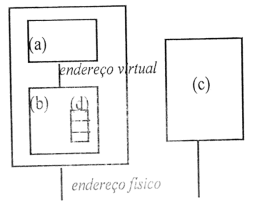
\includegraphics[width=0.4\textwidth]{ex-mem-structure}
    \end{figure}
  }

  \begin{enumerate}[label=(\alph*)]
    \item \textbf{CPU:} envia o endereço virtual à MMU;

    \item \textbf{MMU:} quebra o endereço virtual em duas partes, sendo elas a página e o deslocamento. A MMU usa $p$ como índice na TLB para obter o \textit{frame} $f$. A MMU troca a página $p$ pelo frame $f$, que é inserido no barramento junto com o deslocamento, gerando endereço físico.

    \item \textbf{Memória RAM:} entidade que contém dado desejado. Dado um endereço físico, ela acessa dado;

    \item \textbf{TLB:} \textit{buffer} contido na MMU que possui as últimas entradas referenciadas da tabela de página. Recebe a página como índice para retornar a entrada correspondente, contendo o \textit{frame}.
  \end{enumerate}
\end{exercicio}


\begin{exercicio}
  {2º/2017}{Paginação}
  {Considere um sistema com 4 \textit{frames} e 8 páginas. Admita a seguinte \textit{string} de referência: 0172327103. Quantos \textit{page faults} ocorrerão se o algorítmo de substituição for FIFO? E se for LRU?}
  \label{ex:pagination-1}

  Fazer o exercício de forma a mostrar cada iteração e o histórico das tabelas.

  \textbf{FIFO:} 6 \textit{page faults} \\
  1ª forma: Estado de Memória e Ordem de Saída
  \[
  \begin{array}{rcccccccccc}
    \text{Página Referênciada}
    & 0 & 1 & 7 & 2 & 3 & 2 & 7 & 1 & 0 & 3 \\ \hline
    \text{Resultado}
    & P & P & P & P & P & - & - & - & P & - \\
    \\
    \text{Estado da Memória}
    & 0 & 0 & 0 & 0 & 3 & 3 & 3 & 3 & 3 & 3 \\
    & - & 1 & 1 & 1 & 1 & 1 & 1 & 1 & 0 & 0 \\
    & - & - & 7 & 7 & 7 & 7 & 7 & 7 & 7 & 7 \\
    & - & - & - & 2 & 2 & 2 & 2 & 2 & 2 & 2 \\
    \\
    \text{Ordem de saída}
    & 0 & 1 & 7 & 2 & 3 & 3 & 3 & 3 & 0 & 0 \\
    & - & 0 & 1 & 7 & 2 & 2 & 2 & 2 & 3 & 3 \\
    & - & - & 0 & 1 & 7 & 7 & 7 & 7 & 2 & 2 \\
    & - & - & - & 0 & 1 & 1 & 1 & 1 & 7 & 7 \\
  \end{array}
  \]
2ª forma: Tabela
\[
\begin{array}{rcccccccccc}
  \text{Tempo de referência}
    & 1 & 2 & 3 & 4 & 5 & 6 & 7 & 8 & 9 & 10 \\ \hline
  \text{Página Referênciada}
    & 0 & 1 & 7 & 2 & 3 & 2 & 7 & 1 & 0 & 3 \\ \hline
  \text{Resultado}
    & P & P & P & P & P & - & - & - & P & - \\
\end{array}
 \]
\begin{table}[H]
  \centering
  \begin{tabular}{lll}
    \hline \hline
    \textbf{Frame}  & \textbf{Página}                   & \textbf{Tempo de carga} \\ \hline
    0               & \sout{0} 3                        & \sout{1} 5 \\
    1               & \sout{1} 0                        & \sout{2} 9 \\
    2               & 7                                 & 3 \\
    3               & 2                                 & 4 \\
    \hline \hline
  \end{tabular}
\end{table}

  \textbf{LRU:} 7 \textit{page faults} \\

  1ª forma: Estado de Memória e Ordem de Saída
  \[
  \begin{array}{rcccccccccc}
    \text{Página Referênciada}
    & 0 & 1 & 7 & 2 & 3 & 2 & 7 & 1 & 0 & 3 \\ \hline
    \text{Resultado}
    & P & P & P & P & P & - & - & - & P & P \\
    \\
    \text{Estado da Memória}
    & 0 & 0 & 0 & 0 & 3 & 3 & 3 & 3 & 0 & 0 \\
    & - & 1 & 1 & 1 & 1 & 1 & 1 & 1 & 1 & 1 \\
    & - & - & 7 & 7 & 7 & 7 & 7 & 7 & 7 & 7 \\
    & - & - & - & 2 & 2 & 2 & 2 & 2 & 2 & 3 \\
    \\
    \text{Ordem de saída}
    & 0 & 1 & 7 & 2 & 3 & 2 & 7 & 1 & 0 & 3 \\
    & - & 0 & 1 & 7 & 2 & 3 & 2 & 7 & 1 & 0 \\
    & - & - & 0 & 1 & 7 & 7 & 3 & 2 & 7 & 1 \\
    & - & - & - & 0 & 1 & 1 & 1 & 3 & 2 & 7 \\
  \end{array}
  \]

2ª forma: Tabela
\[
\begin{array}{rcccccccccc}
  \text{Tempo de referência}
    & 1 & 2 & 3 & 4 & 5 & 6 & 7 & 8 & 9 & 10 \\ \hline
  \text{Página Referênciada}
    & 0 & 1 & 7 & 2 & 3 & 2 & 7 & 1 & 0 & 3 \\ \hline
  \text{Resultado}
    & P & P & P & P & P & - & - & - & P & P \\
\end{array}
 \]
\begin{table}[H]
  \centering
  \begin{tabular}{lll}
    \hline \hline
    \textbf{Frame}  & \textbf{Página}                   & \textbf{Tempo de referência} \\ \hline
    0               & \sout{0} \sout{3} 0               & \sout{1} \sout{5} 9 \\
    1               & 1                                 & \sout{2} 8 \\
    2               & 7                                 & \sout{3} 7 \\
    3               & \sout{2} 3                        & \sout{4} \sout{6} 10 \\
    \hline \hline
  \end{tabular}
\end{table}

\end{exercicio}

\begin{exercicio}
  {2º/2017}{Estruturação de Sistemas Operacionais}
  {Explique a estruturação em camadas de sistema operacional. Comente vantagens e desvantagens.}

  SO fica em modo protegido e seu código é distribuído em diversas camadas funcionais, de modo que rotinas de uma camada podem fazer chamadas às camadas imediatamente superior ou inferior.

  \textsc{Vantagens}:
  \begin{enumerate}
    \item Facilidade de manutenção;
    \item Modularidade;
  \end{enumerate}

 \textsc{Desvantagens}:
  \begin{enumerate}
    \item Overhead em relação ao monolítico;
  \end{enumerate}
\end{exercicio}

\begin{exercicio}
  {2º/2017}{Escalonamento de Processos}
  {Considere o conjunto de $6$ processos e respectivos tempos de execução (quantum = $4 ms$). A ordem de chegada dos processos foi $A \rightarrow B \rightarrow C \rightarrow D \rightarrow E \rightarrow F$ (do mais antigo para o mais recente). No momento de início de execução do algoritmo de escalonamento, todos os processos estão prontos. Diga a ordem na qual este conjunto será executado, considerando as políticas \textit{Round-Robin}, \textit{First Come First Served} e \textit{Shortest Job First (SJF)}.
  \begin{table}[H]
    \centering
    \begin{tabular}{cc}
      \hline \hline
      \textbf{Processo} & \textbf{Tempo de execução (ms)} \\ \hline
      A                 & 9                               \\
      B                 & 10                              \\
      C                 & 2                               \\
      D                 & 6                               \\
      E                 & 8                               \\
      E                 & 3                              \\ \hline \hline
    \end{tabular}
  \end{table}.}

  \textbf{Round-robin:} $A \rightarrow B \rightarrow C \rightarrow D \rightarrow E \rightarrow F \rightarrow A \rightarrow B \rightarrow D \rightarrow E \rightarrow A \rightarrow B$

  \textbf{SJF:} $C \rightarrow F \rightarrow D \rightarrow E \rightarrow A \rightarrow B$

  \textbf{FCFS:} $A \rightarrow B \rightarrow C \rightarrow D \rightarrow E \rightarrow F$
\end{exercicio}

\begin{exercicio}
  {2º/2017}{Arquiteturas de SO/Processos}
  {Cite os passos para a criação de processos nas arquiteturas monolíticas, \textit{microkernel} e \textit{exokernel}.}
  \label{ex:processes-creation}

  Para as \textsc{arquiteturas monolíticas}:
  \begin{enumerate}
    \item O processo pai solicita a criação de um processo filho, através de uma \textit{chamada de sistema} \texttt{create process};

    \item O SO aloca uma entrada livre na \textit{tabela de processos} para o processo filho;

    \item O SO atribui um \textit{PID} ao processo filho;

    \item O SO ajusta a \textit{área de memória} para a execução do processo filho;

    \item O SO preenche os \textit{valores de registradores} para execução do processo filho na tabela de processos;

    \item O SO insere o processo filho na fila \textit{ready} do escalonador;

    \item O SO retorna ao processo pai.
  \end{enumerate}

  Para o \textsc{microkernel}:
  \begin{enumerate}
    \item O processo pai envia uma mensagem para o microkernel, colocando o \texttt{create process} como conteúdo;

    \item O microkernel recebe a mensagem e determina que o processo filho deve ser criado;

    \item O microkernel aloca uma entrada livre na \textit{tabela de processos} para o processo filho;

    \item O microkernel atribui um \textit{PID} ao processo filho;

    \item O microkernel ajusta a \textit{área de memória} para a execução do processo filho;

    \item O microkernel preenche os \textit{valores de registradores} para execução do processo filho na tabela de processos;

    \item O microkernel insere o processo filho na fila \textit{ready} do escalonador;

    \item O microkernel envia uma mensagem para o processo pai contendo o valor de retorno.
  \end{enumerate}

  Para o \textsc{exokernel}:
  \begin{enumerate}
    \item O processo pai solicita a criação de um processo filho para a LibOS, através de uma \textit{chamada de função} \texttt{create process};

    \item A LibOS aloca uma entrada livre na \textit{tabela de processos} para o processo filho;

    \item A LibOS atribui um \textit{PID} ao processo filho;

    \item A LibOS pede uma região de software (área de memória) ao exokernel, via \textit{chamada de sistema}. Esta área é destinada ao processo filho;

    \item A LibOS solicita um \textit{processor environment} (PE), via chamada de sistema, e copiar o valor dos registradores para lá;

    \item A LibOS preenche o de prólogo e epílogo do PE (troca de contexto), descarregando o código;

    \item O exokernel coloca o PE na sua fila \textit{ready};

    \item A LibOS coloca o processo na sua fila \textit{ready};

    \item A LibOS retorna ao processo pai.
  \end{enumerate}

\end{exercicio}

\begin{exercicio}
  {2º/2017}{Memória (Paginação)}
  {Tendo a tabela de páginas abaixo e recebendo o endereço $12$, que endereço a MMU vai colocar no barramento? (Considere páginas de 1KBytes)
  Faça o mesmo exercício para o endereço $3150$.
  \begin{table}[H]
    \centering
    \caption{Look-Aside Buffer Table}
    \label{tab:pag_to_frame}
    \begin{tabular}{cc}
      \hline \hline
    Página & Frame \\ \hline
    0      & 2     \\
    1      & 1     \\
    2      & 0     \\
    3      & 5     \\ \hline \hline
    \end{tabular}
    \end{table}}

    1. Para endereço $X$ divide-se o endereço pelo tamanho da página, e encontra-se a página requerida.
    2. Após isto pega-se o número do frame e multiplica-se pelo tamanho para encontrar o endereço da página, soma-se o deslocamento (resto da divisão do primeiro passo).

    Para $12$, 12/1024 = 0, resto 12. Página 0 é o frame 2, 2 * 1024 = 2048, 2048 + 12 = 2060.
    Para $3150$, 3150/1024 = 3, resto 78. Página 3 é o frame 5, 5 * 1024 = 5120, 5120 + 78 = 5198.
\end{exercicio}
